%======================================================================
\section{Results}
\label{sec:results}
%======================================================================
All 54 E1 runs completed successfully (success rate $1.00$ for every cell); no provider timeouts or schema-parse failures occurred with constrained decoding. Table~\ref{tab:main} and Fig.~\ref{fig:main} summarise ground-truth outcomes.

\begin{table*}[t]
\centering
\caption{E1 end-to-end results (mean over 3 repetitions; $\pm$ is s.d.). \emph{Recall}: correctly repaired / injected corruptions (S2: fraction of injected duplicates removed). \emph{C/I/U}: correctly repaired, incorrectly repaired, unrepaired cells. \emph{Dmg}: originally clean cells modified. \emph{Issues}: comparator's detected issue count before$\to$after (an observed signal, not correctness). \emph{Time}: strategy wall time in seconds, including the LLM call.}
\label{tab:main}
\footnotesize
\begin{tabular}{@{}llcccccr@{}}
\toprule
\textbf{Scen.} & \textbf{Arm} & \textbf{Recall} & \textbf{C/I/U} & \textbf{Dmg} & \textbf{FMR} & \textbf{Issues} & \textbf{Time}\\
\midrule
\tabinput{../tables/main_results.tex}
\bottomrule
\end{tabular}
\end{table*}

\begin{figure*}[t]
\centering
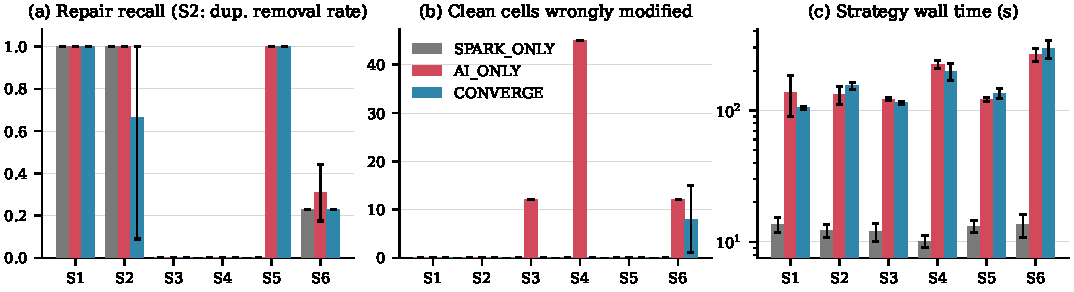
\includegraphics[width=\textwidth]{main_results.pdf}
\caption{E1 results by scenario and arm. (a) Ground-truth repair quality; (b) collateral damage to originally clean cells; (c) strategy wall time (log scale). AI is necessary for date and categorical semantics (S5), but unvalidated AI causes all of the large collateral damage (S3, S4).}
\label{fig:main}
\end{figure*}

\subsection{RQ1: Does AI Improve Repair Quality?}
\label{sec:res-rq1}
\emph{Where the corruption requires a semantic decision and the model makes the right one, yes---decisively.} On S5 (mixed date formats) the deterministic baseline, which by design refuses to choose a target format, leaves all three corrupted dates unrepaired (recall $0.00$), whereas both AI arms choose \texttt{STANDARDIZE\_DATE\_FORMAT} with target \texttt{YYYY-MM-DD} in every repetition and restore all three cells exactly (recall $1.00$, zero collateral damage).

\emph{Where the corruption is mechanically determined, AI adds nothing.} On S1 all three arms reach recall $1.00$; as discussed in \S\ref{sec:discussion}, this is partly an artefact of Spark's CSV writer, which trims whitespace on output, as the no-op control in E2 confirms. On S2 the baseline and \textsc{AI\_Only} both remove both injected duplicates without losing an original row.

\emph{Where the corruption is information-theoretically unrecoverable, no arm succeeds.} On S4 the true salaries cannot be derived from aggregates; \textsc{AI\_Only}'s mean imputation produces two \emph{incorrect} repairs, while \textsc{Spark\_Only} and \textsc{Converge} leave the cells missing.

\emph{Where the model's judgement is wrong, AI makes things worse.} On S3 the model consistently proposed \texttt{NORMALIZE\_CASE(lower)} on \texttt{department} rather than a canonicalising \texttt{STANDARDIZE\_CATEGORY}. Lowercasing does unify the variant groups, but toward a value (\texttt{engineering}) that disagrees with the twelve correct cells. On S6 the model's plan varied between repetitions (consistency $0.67$) and achieved mean recall $0.31\pm0.13$ under \textsc{AI\_Only}, versus $0.23$ for the baseline.

\subsection{RQ2: Does Validation Reduce Hallucination-Driven Errors?}
\label{sec:res-rq2}
Collateral damage (Fig.~\ref{fig:main}b) answers RQ2 most directly. Unvalidated AI modified \textbf{12} clean cells on S3, \textbf{45} on S4 (FMR $0.51$: the model invented whitespace and casing problems on \texttt{name}, \texttt{department} and \texttt{city} for which the profiler had produced no evidence, and lowercased all three columns), and \textbf{12} on S6. Under \textsc{Converge} the damage was \textbf{0} on S4, where all three fabricated recommendations were rejected for lack of evidence (\texttt{evidence\_exists}) or an ill-typed parameter, and \textbf{0} on S3. Summed over the six scenarios, mean collateral damage per run fell from $69$ to $8$ cells ($-88\%$), while every correct repair the model produced on S1 and S5 was preserved. The audit below shows, however, that the S3 outcome must be attributed with care: two of the three S3 rejections stem from a validator defect, and with that defect corrected the S3 recommendation would have been \emph{approved} and would have caused the same 12-cell damage. Under the corrected validator the reduction is therefore $69\to20$ cells ($-71\%$)---still substantial, and entirely due to evidence checks that worked as designed (S4).

The comparator's observed signals (Table~\ref{tab:main}, \emph{Issues}) are instructive: by that measure \textsc{AI\_Only} looks \emph{best} on S3 and S4 (all detected issues resolved, $2\to0$ and $1\to0$), precisely where it inflicted the most damage. Lowercasing every value removes the variant groups the profiler detects, and imputation removes the null count. This vindicates the decision to never merge observed issue counts with ground-truth correctness (ADR-009): \emph{an AI cleaning system evaluated only by downstream data-quality checks can appear to succeed while corrupting the data}.

\subsection{Recommendation-Level Audit}
\label{sec:res-audit}
Across the 18 \textsc{Converge} runs the model produced 35 recommendations (Table~\ref{tab:audit}). The validator approved 15 (13 \textsc{safe}, 2 \textsc{review}) and rejected 20: 6 for absent evidence (fabricated issues), 8 for contradicted claims, and 6 for an ill-typed parameter (\texttt{fill\_value: null} on a mean imputation). Manual inspection of every verdict against ground truth reveals three distinct failure modes of the \emph{validator}, each of which we consider a contribution of the audit:

\begin{enumerate}[leftmargin=*,nosep]
  \item \textbf{Evidence-ambiguity false rejections (3 of 20).} When the profiler emits several evidence items with the same issue type and column (two variant groups for \texttt{department}; two duplicate groups on S2), the claim check compares the model's claimed values against only the \emph{first} matching item. A correct claim about the second group (e.g., duplicate pair R011/R016, which the ground-truth manifest confirms) is then reported as a contradiction. An offline re-validation with a corrected ``any-matching-item'' rule flips exactly these three verdicts. The consequences are mixed: on S2 the false rejection cost one repetition both duplicate removals, whereas on S3 it \emph{accidentally} blocked a harmful lowercasing---a reminder that a validator's apparent wins must be audited as carefully as its losses.
  \item \textbf{Over-strict optional parameters (6 of 20).} Every \texttt{FILL\_MISSING} recommendation passed \texttt{fill\_value: null} for an optional parameter and was rejected on type; this is conservative but harmless here, since any imputation is an incorrect repair under exact ground truth.
  \item \textbf{Evidence-type conflation (2 approvals).} On S6, \texttt{NORMALIZE\_CASE(lower)} on \texttt{name} was \emph{approved} because the catalog lets \texttt{whitespace\_or\_casing} evidence justify a case change; the profiler had flagged only whitespace. All 12 clean names were lowercased. This is the source of \textsc{Converge}'s residual damage on S6 and shows that \emph{the validator is only as strong as the evidence requirements declared in its catalog}.
\end{enumerate}
Conversely, the validator also rejected a recommendation that would have been beneficial: on S6 repetition 0 the model proposed the correct date standardisation but claimed \texttt{\{YYYY-MM-DD: 14\}} for a column whose real histogram contained two formats; the contradicted claim cost three correct repairs. We regard this as correct behaviour---a recommendation whose stated evidential basis is false should not execute unattended---but it quantifies the conservativeness cost of evidence validation.

\begin{table}[t]
\centering
\caption{E1 audit of all 35 LLM recommendations under \textsc{Converge}.}
\label{tab:audit}
\footnotesize
\begin{tabular}{@{}lrl@{}}
\toprule
\textbf{Validator outcome} & \textbf{n} & \textbf{Ground-truth assessment}\\
\midrule
Approved, \textsc{safe} tier & 13 & 11 beneficial, 2 harmful (conflation)\\
Approved, \textsc{review} tier & 2 & beneficial (S2 dedup)\\
Rejected: no evidence & 6 & all fabricated issues (S4)\\
Rejected: contradicted claim & 8 & 5 genuinely false, 3 ambiguity\\
Rejected: parameter type & 6 & \texttt{fill\_value: null}\\
\bottomrule
\end{tabular}
\end{table}
